\documentclass{beamer}
\usetheme{Berkeley}
%\usetheme{Copenhagen}
%\usecolor{default}

\usepackage{etex}
\usepackage[usenames,dvipsnames]{pstricks}
\usepackage{amsfonts}
\usepackage{amsmath}
\usepackage{amssymb}
\usepackage{epsfig}
\usepackage{graphicx}
\usepackage{mathrsfs}
%\usepackage{pst-grad} % For gradients
%\usepackage{pst-plot} % For axes
\usepackage{subcaption}
\usepackage{tikz}
\usepackage{tkz-graph}
%\usepackage{fancyhdr}
\usepackage{algorithm}
\usepackage{algorithmic}
\usepackage{url}

\usetikzlibrary{arrows, shapes}

\title{Estimation on Graphs From Relative Measurements}
\subtitle{A Paper by Prabir Barooah and Jo\~{a}o P. Hespanha}
\author{Presented by Mark Edwards}%\\Based on a paper by Prabir Barooah and
%Jo\~{a}o P. Hespanha}
\institute{\url{mark.edards727@myci.csuci.edu}\\
    University of California Channel Islands}
\date{\today}


\begin{document}

\begin{frame}
\titlepage
\end{frame}

\begin{frame}
\begin{figure}[c]
\includegraphics[width=\textwidth]{building-consensus-banner.jpg}
\end{figure}
\end{frame}

\setbeamertemplate{footline}[frame number]

\begin{frame}{Overview}
\tableofcontents % Print the title page as the first slide.
\nocite{barooah}
\end{frame}

\section{Relative Measurements}
\begin{frame}{Relative Measurements}
\begin{center}
\emph{Relative Measurements} are sensor readings taken relative to other nodes
in a sensor network
\end{center}
\end{frame}

\begin{frame}{Relative Measurements}
\begin{center}
Relative Measurements are \emph{NOT}
\begin{itemize}
\item<1-> Absolute Position (GPS)
\item<2-> Absolute Temperature (Thermometer Sensor)
\item<3-> Absolute Velocity (Accelerometer)
\end{itemize}
\end{center}
\end{frame}

\begin{frame}{Relative Measurements}
\begin{center}
Relative Measurements \emph{ARE}
\begin{itemize}
\item Relative Position from Heading and Bearing
\end{itemize}
\end{center}
\end{frame}

\begin{frame}{Relative Measurements}
  \begin{columns}[T]
    \begin{column}{.5\textwidth}
     \begin{block}{Relative Position}
        \begin{itemize}
            \item Heading measured using Compass Sensor
            \item Distance measured using Optical Sensor
            \item We want relative Cartesian displacement 
        \end{itemize}
% Your text here
    \end{block}
    \end{column}
    \begin{column}{.5\textwidth}
    \begin{block}{Example}
% Your image included here
    \includegraphics[width=\textwidth]{relative_position.png}
    \end{block}
    \end{column}
  \end{columns}
\end{frame}

\begin{frame}{Relative Measurements}
  \begin{columns}[T]
    \begin{column}{.5\textwidth}
     \begin{block}{Relative Position}
        \begin{itemize}
            \item Let $w$ be our reference ``master''
            \item Let $\theta_{u,v} = 30^{\circ}, d_{u,v} = 1$ $\theta_{v,w} =
            60^{\circ}, d_{v,w} = 1$
            \item Then $u$ is at $\left(-\frac{\sqrt{3}+1}{2},
            -\frac{\sqrt{3}+1}{2}\right)$
        \end{itemize}
% Your text here
    \end{block}
    \end{column}
    \begin{column}{.5\textwidth}
    \begin{block}{Example}
% Your image included here
    \includegraphics[width=\textwidth]{relative_position.png}
    \end{block}
    \end{column}
  \end{columns}
\end{frame}

\begin{frame}{Relative Measurements}
\begin{center}
Relative Measurements \emph{ARE}
\begin{itemize}
\item Relative Position from Heading and Bearing
\item Time-Synchronization 
\end{itemize}
\end{center}
\end{frame}

\begin{frame}{Relative Measurements}
\begin{columns}[T]
    \begin{column}{.5\textwidth}
     \begin{block}{Time-Synchronization}
        \begin{itemize}
            \item We want to synchronize time between $u$ and ``master node''
            $w$ 
            \item We want to update $u$ to $t_u = t_u + (t_v - t_u) + (t_w -
            t_v)$ 
        \end{itemize}
% Your text here
    \end{block}
    \end{column}
    \begin{column}{.5\textwidth}
    \begin{block}{Example}
% Your image included here
    \includegraphics[width=\textwidth]{relative_time.png}
    \end{block}
    \end{column}
  \end{columns}
\end{frame}

\begin{frame}{Relative Measurements}
\begin{center}
Relative Measurements \emph{ARE}
\begin{itemize}
\item Relative Position from Heading and Bearing
\item Time-Synchronization 
\item Relative Velocity
\end{itemize}
\end{center}
\end{frame}

\begin{frame}{Relative Measurements}
  \begin{columns}[T]
    \begin{column}{.5\textwidth}
     \begin{block}{Relative Velocity}
        \begin{itemize}
            \item Let $w$ be our reference ``master''
            \item We track relative position over time to get velocity
            \item We want $\dot{u} = \dot{u} + (\dot{v} - \dot{u}) + (\dot{w} -
            \dot{v})$ 
        \end{itemize}
% Your text here
    \end{block}
    \end{column}
    \begin{column}{.5\textwidth}
    \begin{block}{Example}
% Your image included here
    \includegraphics[width=\textwidth]{relative_position.png}
    \end{block}
    \end{column}
  \end{columns}
\end{frame}

\begin{frame}{Relative Measurements}
A few points:
\begin{itemize}
\item The preceding graphs are \emph{Measurement Graphs} not \emph{Connectivity
Graphs}
\item We implicitly assume bi-directional communication between all nodes that
share a measurement edge. 
\end{itemize}
\end{frame}

\begin{frame}{Relative Measurements}
\begin{center}
Each ``hop'' in a measurement graph is a measurement $\zeta$ with some error
$\epsilon$
%\tikzstyle{vertex}=[circle,fill=black!25,minimum size=20pt,inner sep=0pt]
%\tikzstyle{edge} = [draw,thick,->]
\begin{figure}
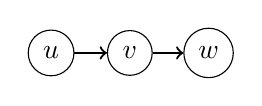
\begin{tikzpicture}
\node[circle, draw] (u) at (0,0) {$u$};
\node[circle, draw, right of=u] (v) {$v$};
\node[circle, draw, right of=v] (w) {$w$};
\path [draw, thick, ->] (u) -- (v); %{$\epsilon_{u,v}$};
\draw [draw, thick, ->] (v) -- (w);% {$\epsilon_{v,w}$};
\end{tikzpicture}
\end{figure}
\[ \zeta_{u,v} = u - v + \epsilon_{u,v}, \zeta_{v,w} = v - w + \epsilon_{v,w} \]
\end{center}
\end{frame}

\begin{frame}{Relative Measurements}
\begin{center}
This can be written in ``matrix form'' as
\[ \mathbf{z} - \mathcal{A}_r^T\mathbf{x}_r = \mathcal{A}_b^T \mathbf{x} +
 \epsilon \]
 \begin{itemize}
 \item $\mathbf{z}$ are the measurements
 \item $\mathcal{A}_r$ is the incidence
 matrix for the reference nodes $\mathbf{x}_r$
 \item $\mathcal{A}_b$ is the incidence
 matrix for unknown nodes $\mathbf{x}$ 
 \item $\epsilon$ is still the error.
 \end{itemize}
 \end{center}
 \end{frame}

 \begin{frame}{Relative Measurements}
 \begin{center}
 We may also define the covariance matrix $\mathcal{P}$ as
 \[ P := E[\epsilon \epsilon^T] \]
Since we assume that $\epsilon$ is a random vector with zero mean. 
\end{center}
\end{frame}

 \begin{frame}{Relative Measurements}
 \begin{center}
 And based on this, we can now apply least squares to get the \emph{Best Least
 Unbiased Estimator}
 \[ \hat{\mathbf{x}}^{*} := \mathcal{L}^{-1} \mathbf{b} \]
 Where
 \[ \mathcal{L} :=\mathcal{A}_b \mathcal{P}^{-1} \mathcal{A}_b^T \]
 \[ b := \mathcal{A}_b \mathcal{P}^{-1} \left( \mathbf{z} - \mathcal{A}_r^T
 \mathbf{x}_r \right ) \]
  \end{center}
\end{frame}

\begin{frame}{Relative Measurements}
\begin{center}
We may also
\[ \Sigma :=
 E[(\mathbf{x}-\hat{\mathbf{x}}^{*})(\mathbf{x}-\hat{\mathbf{x}}^{*})^T] =
 \mathcal{L}^{-1} \]
 \end{center}
 \end{frame}


\begin{frame}{Relative Measurements}

\begin{center}
For this particular graph, we see that error scales linearly with respect to the
number of nodes
\begin{figure}
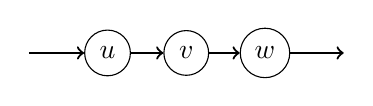
\begin{tikzpicture}
\node[circle, draw] (u) at (1,0) {$u$};
\node[circle, draw, right of=u] (v) {$v$};
\node[circle, draw, right of=v] (w) {$w$};
\draw [draw, thick, ->] (0,0) -- (u);
\draw [draw, thick, ->] (u) -- (v); %{$\epsilon_{u,v}$};
\draw [draw, thick, ->] (v) -- (w);% {$\epsilon_{v,w}$};
\draw [draw, thick, ->] (w) -- (4,0);
\end{tikzpicture}
\end{figure}
\[ \epsilon_{u,w} = \epsilon_{u,v} + \epsilon_{v,w} \]
\[ \epsilon_{i,j} = \sum_{k = i}^{j-1} \epsilon_{k,k+1} \]
\end{center}
\end{frame}

\begin{frame}{Relative Measurements}

\begin{center}
This begets the question, ``can we more generally put a lower bound on our
error''?
\pause
\vspace{5mm}

Yes!
\end{center}
\end{frame}

\section{Error Bounds}
\begin{frame}{Error Bounds}
\begin{center}
In order to address error bounds, we need a way to address structure within the
graph.
\pause
\vspace{5mm}

A traditional method of quantifying the structure of a graph is with the degrees
of each node.
\end{center}
\end{frame}


\begin{frame}{Error Bounds}
\begin{center}
But this doesn't work\ldots
\begin{figure}
\begin{subfigure}[c]{0.3\textwidth}
\includegraphics[width=\textwidth]{linear_degree_6.png}
\caption{Linear Error Scaling}
\end{subfigure}
\begin{subfigure}[c]{0.3\textwidth}
\includegraphics[width=\textwidth]{logarithmic_degree_6.png}
\caption{Logarithmic Error Scaling}
\end{subfigure}
\begin{subfigure}[c]{0.3\textwidth}
\includegraphics[width=\textwidth]{constant_degree_6.png}
\caption{Constant Error Scaling}
\end{subfigure}
\end{figure}
\end{center}
\end{frame}

\begin{frame}{Error Bounds}
\begin{center}
In order to more directly measure structure, we define the concept of an
\emph{embedding}
\includegraphics[width=0.9\textwidth]{graph_embedding.png}
\end{center}
\end{frame}

\begin{frame}{Error Bounds}
\begin{center}
And the concept of a \emph{lattice}
\includegraphics[width=0.9\textwidth]{lattice_overview.png}
\end{center}
\end{frame}

\begin{frame}{Error Bounds}
\begin{center}
And make the following claims with respect to the number of nodes:
\begin{itemize}
\item<1-> A 1D lattice has error that scales linearly
\item<2-> A 2D lattice has error that scales logarithmically 
\item<3-> A 3D lattice has error that is constant with respect to the number of
nodes!
\end{itemize}
\end{center}
\end{frame}

\begin{frame}{Error Bounds}
\begin{center}
Finally, we generalize this using embeddings by noting that if a graph $G$ is
embedded in another graph $\bar{G}$, that the error $G$ is at least that of
$\bar{G}$
\pause
\vspace{5mm}
\\
With this, we now turn to estimation methods that approach these error bounds.
\end{center}
\end{frame}

\section{Jacobi Iteration}
\begin{frame}{Jacobi Iteration}
Jacobi Iteration is an algorithm we inherit from Linear Algebra. 
\pause
\vspace{5mm}
\\
Intuitively, it
can be understood as ``guess and check''
\end{frame}

\begin{frame}{Jacobi Iteration}
In layman's terms, the algorithm is
\begin{enumerate}
\item<1-> Arbitrarily guess values for 1 hop neighbors.
\item<2-> At the $i$th iteration, use the current estimates of 1 hop neighbors to
estimate each node's current value. Each node then broadcasts it's estimate of its own value
to all its 1 hop neighbors. 
\item<3-> At the end of the $i$th iteration, each node then uses the broadcasted
estimates for the $i+1$st iteration. 
\end{enumerate}
\end{frame}

\begin{frame}{Jacobi Iteration}
\begin{center}
Mathematically, the second step involves solving 
\[ \left(\sum_{e \in E_u} P_e^{-1}\right) \hat{x}_u^{(i+1)} = \sum_{e \in E_u}
P_e^{-1} \left( \hat{x}^{(i)}_{v_e} +a_{ue}\zeta_e \right) \]
for 
\[ \hat{x}_u^{(i+1)} \]
%where 
\end{center}
\end{frame}

\begin{frame}
\begin{center}
Intuitively this systematically uses the measurements to update our estimate,
which is then filtered by the covariance matrix. 
\end{center}
\end{frame}


\begin{frame}{Jacobi Iteration}
\begin{center}
The Jacobi Iteration method approaches the optimal estimate, scales, and is
robust to temporary link failures. 
\pause
\vspace{5mm}
\\
However, its convergence rate is relatively slow. 
\end{center}
\end{frame}

\section{Overlapping Subgraph Estimator (OSE)}
\begin{frame}{Overlapping Subgraph Estimator}
The Overlapping Subgraph Estimator (OSE) algorithm extends the Jacobi method.
\begin{itemize}
\item<1-> Instead of each node sending only their estimates of their own values, each node
sends both their own estimates and the estimates received.
\item<2-> This essentially enables 2-hop communication. 
\item<3-> While each node in the Jacobi method only considers its immediate
neighbors, the nodes in the OSE algorithm see themselves as the center of their
own 2 hop graph. 
\end{itemize}
\end{frame}

\begin{frame}{Overlapping Subgraph Estimator}
The OSE algorithm follows the following steps. For a given node $u$, 
\begin{enumerate}
\item<1-> Generate an arbitrary guess for the values of the 2-hop neighbors of
$u$
\item<2-> Get estimates for each node in the 1 hop neighborhood of $u$ based on the least squares
of the estimates of the 2-hop neighbors. 
\item<3-> Perform a weighted average between the previous value for $u$ and the
value for $u$ generated in step 2. Broadcast this new value as well as the
previously received values for the 1-hop neighbors.
\item<4-> Listen for updates from the 1-hop neighbors and update estimates for
2-hop neighbors. Repeat steps 2--4 as needed.
\end{enumerate}
\end{frame}

\begin{frame}{Overlapping Subgraph Estimator}
While the OSE algorithm as previously described examines a 2-hop radius, the
radius can be made arbitrarily large. However, this requires much more
communication bandwidth, with diminishing marginal benefit.
\end{frame}

\section{Conclusions}
\begin{frame}{Conclusions}
\begin{center}
To compare the convergence of both the Jacobi and the OSE methods, consider the
following test.
\begin{itemize}
\item<1-> 200 nodes separated by a distance less than 0.11
\item<2-> Perform the bearing, range test mentioned previously.
\item<2-> Add Guassian noise with $\sigma = 0.0165$ for radial distance and
$\sigma = 10^{\circ}$ for bearing.
\end{itemize}
\end{center}
\end{frame}
\begin{frame}{Conclusions}
\begin{center}
\includegraphics[width=0.7\textwidth]{comparison.png}
\end{center}
\end{frame}

\section*{Questions}
\begin{frame}
Questions?
\end{frame}

\begin{frame}{References}%[allowframebreaks]
\bibliographystyle{unsrt}
\bibliography{final_project}
\end{frame}


%Sensor node have local partial knowledge. In particular, they have access to a
%comparative measurement \emph{between} connected nodes. This is not to be
%confused with the agreement protocol or ``temperature measurments.'' This
%referrs only to mesurements taken between two points, such as time or relative
%position. 
%\[ \zeta_{u,v} = p_u - p_v + \epsilon_{u,v} \]
%
%For a very simple example of a path graph, the lowest limit of error scales
%linearly with respect to the number of nodes. The authors show that this can be
%improved to a logarithmic upper bound  for many types of graphs. 
%
%Since this field is so new, we draw things from many exsiting fields. For
%finding the boundries of algorithms, we draw from Electrical Engineering. For
%finding algorithms, we draw analogies and take inspiration from parallel programming.
%
%From our basic definitions of variance and estimation, we see that the Best
%Linear Unbiased Estimate is generated by the Least Squares algorithm and is 
%\[ \mathbf{z} = \mathcal{A}^{T} \mathbf{x} + \epsilon \]
%\[ \mathbf{z} - \mathcal{A}_r^T\mathbf{x}_r = \mathcal{A}_b^T \mathbf{x} +
%\epsilon \]
%\[ \hat{\mathbf{x}}^{*} := \mathcal{L}^{-1} \mathbf{b} \]
%\[ \mathcal{L} :=\mathcal{A}_b \mathcal{P}^{-1} \mathcal{A}_b^T \]
%\[ b := \mathcal{A}_b \mathcal{P}^{-1} \left( \mathbf{z} - \mathcal{A}_r^T
%\mathbf{x}_r \right ) \]
%\[ \Sigma :=
%E[(\mathbf{x}-\hat{\mathbf{x}}^{*})(\mathbf{x}-\hat{\mathbf{x}}^{*})^T] =
%\mathcal{L}^{-1} \]
%
%where $x_r$ referrs to the known reference variables. 
%
%
%In order to tackle these problems, the authors make an analogy to electrical
%resistances in electronic circuits. In fact, for a weakly connected sensor
%Graph, the Best Linear Unbiased Estimate (BLUE) for the varience in both scalar
%and matrix form is the same as the electrical resistance between two points in
%an equivalent electal network. 
%
%From Reylegh's Theorem on Resistances in resistors, we see that adding nodes and
%edges never decreases (only increases) the accuracy of our combined
%measurments. 
%
%From all of this, we derive optimal performance parameters for a graph. In order
%to do this, however, we need one more thing: a graphical way to quanitfy density
%in a graph. Consider the following 3 graphs. All have the same degrees for each
%node, but have different effective errors between distant nodes. 
%




\end{document}
